\chapter{Řízení lidských zdrojů} \label{DBSmanagement}

Řízení lidských zdrojů je jednou z nejobtížnějších součástí projektového řízení, především proto, že se prolíná s dalšími odvětvími jako například \emph{psychologií} či \emph{sociologií}. Jelikož lidé jsou hnací silou projektu, mohou různé metody či samotná kvalita (ba dokonce absence!) řízení lidských zdrojů odrážet výsledný úspěch či neúspěch projektu. I v DBS projektu tedy vyvstala potřeba tuto pozici zaujmout a chopil jsem se jí já, jak již bylo popsáno v kapitole \ref{intro:management}.

\subsection{Role psychologie v řízení lidí}
Ještě než se ponoříme do samotných procesů popisujících řízení lidských zdrojů, věnujme se chvíli právě oněm dalším odvětvím, které se s řízením lidí prolínají. Jak již bylo řečeno, jedná se především o \emph{psychologii}.

Lidé nejsou stroje, kterým bychom poskytli určitý vstup a podle jeho množství mohli očekávat výstup. Je potřeba se zamýšlet nad dalšími okolnostmi, proč pro nás daný člověk pracuje, zda je spokojený, kdy odvádí nejlepší práci atp. Za veškerou lidskou činností stojí \emph{nějaká} motivace, cílem projektového manažera je proto najít, co motivuje právě jemu svěřené pracovníky.

\paragraph{\nameref{picture:maslow}}
\begin{figure}[h]
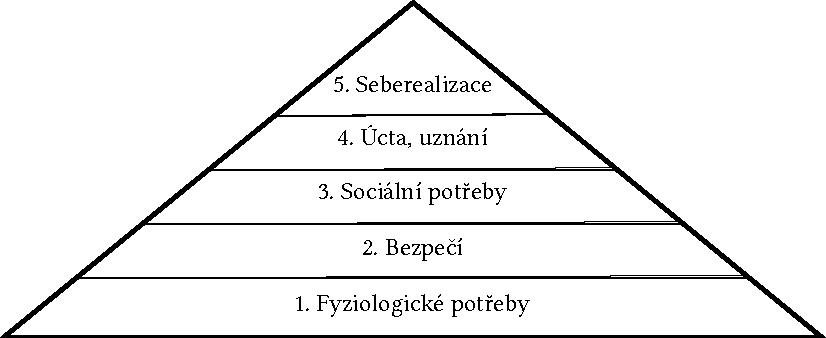
\includegraphics[width=\textwidth]{../pdf/maslow.pdf}
\caption{Maslowova pyramida potřeb} \label{picture:maslow}
\end{figure}

Ve standardních projektech, kde jsou vývojáři odměňováni finančně, se dá plat považovat za splnění základních fyziologických potřeb, protože je za něj možné nakoupit jídlo či pití. V DBS projektu jsou namísto finančně studenti hodnoceni známkou z předmětu, který je pro jejich studijní obor povinný. Jelikož však \emph{vystudování vysoké školy} obecně je spíše potřebou \emph{úcty, uznání} či \emph{seberealizace}, jedná se o vyšší patra pyramidy. Maslow \cite{maslow} tvrdí, že není možné uspokojovat vyšší patra pyramidy, pokud nejsou zajištěny ty nižší. Z toho důvodu může být obtížné motivovat k práci ty studenty, kteří nejprve potřebují vyřešit své zabezpečení (1. a 2. úroveň pyramidy), takoví studenti budou logicky dávat přednost před prací na projektu opravdové práci, za kterou dostanou peníze. Jakmile však má student zajištěny tyto \uv{nižší potřeby}, dostávají se do popředí právě ty, které může DBS projekt nabídnout. Tím se otevírají skvělé možnosti pro rozvoj jak samotných studentů, tak výsledného portálu. Jako příklad uvedu Pavla Kováře, který v tuto chvíli pracuje na bakalářské práci na téma \emph{Automatizované testování webového portálu dbs.fit.cvut.cz}. K projektu se dostal stejnou cestou jako já, ale o rok později. Po dokončení předmětu BI-SP2 se rozhodl u projektu zůstat a pokračovat v jeho vývoji. Jelikož již během vývoje v rámci SP týmů sám od sebe přicházel s inovacemi a kvalitními návrhy na zlepšení, jedná se dle mého názoru o jasný příklad naplňování nejvyšší potřeby, a to \emph{seberealizace}.\\
Právě seberealizace je jedna z potřeb, na kterou se snažím při řízení DBS projektu klást důraz. Studenti jsou hodnoceni jednak za práci, která je jim zadána, zároveň ale dostávají příležitosti rozvíjet vlastní nápady a přínosy projektu a jsou za tyto přínosy také kladně hodnoceni. Více o hodnocení je popisováno v sekci \ref{ppl:ranking}.

\subsection{Procesy řízení lidských zdrojů}

Jak popisuje Schwalbe \cite{schwalbe} ve své knize \emph{Řízení projektů v IT: kompletní průvodce}, při řízení lidských zdrojů se rozeznávají následující procesy:
\begin{itemize}
	\item Vytvoření plánu lidských zdrojů.
	\item Zajištění projektového týmu.
	\item Rozvoj projektového týmu.
	\item Řízení projektového týmu.
\end{itemize}
V následujících sekcích si jednotlivé procesy rozebereme podrobněji a zaměříme se i na jejich roli v DBS projektu.

%%%%%%%%%%%%%%%%%%%%%%%%%%%%%%
%%%%%%%%%%%%%%%%%%%%%%%%%%%%%%
%%%%%%%%%%%%%%%%%%%%%%%%%%%%%%

\section{Vytvoření plánu lidských zdrojů}

Cílem tohoto procesu je vytvořit plán, jaké \emph{typy} lidí potřebujeme do projektu zapojit. Může se jednat například o \emph{profesionálního C++ programátora} či \emph{webdesignéra s citem pro UI a UX} atp. Typicky je vytvořena stromová struktura, kterou zastřešuje projektový manažer a která se dále dělí například na jednotlivé části - programátoři, testeři, grafici, z nichž například programátoři mohou být dále rozděleni do týmů starajících se o jednotlivé komponenty systému, kde každý tým má ještě svého vedoucího. Takovému plánu se říká \emph{OBS} (Organization Breakdown Structure). Tato struktura by měla být vytvořena na začátku projektu a podle ni následně zvoleni vedoucí daných oblastí.

\paragraph{Použití v DBS projektu}
V DBS projektu popisuje organizační členění obrázek \ref{picture:obs}.
\begin{figure}[h]
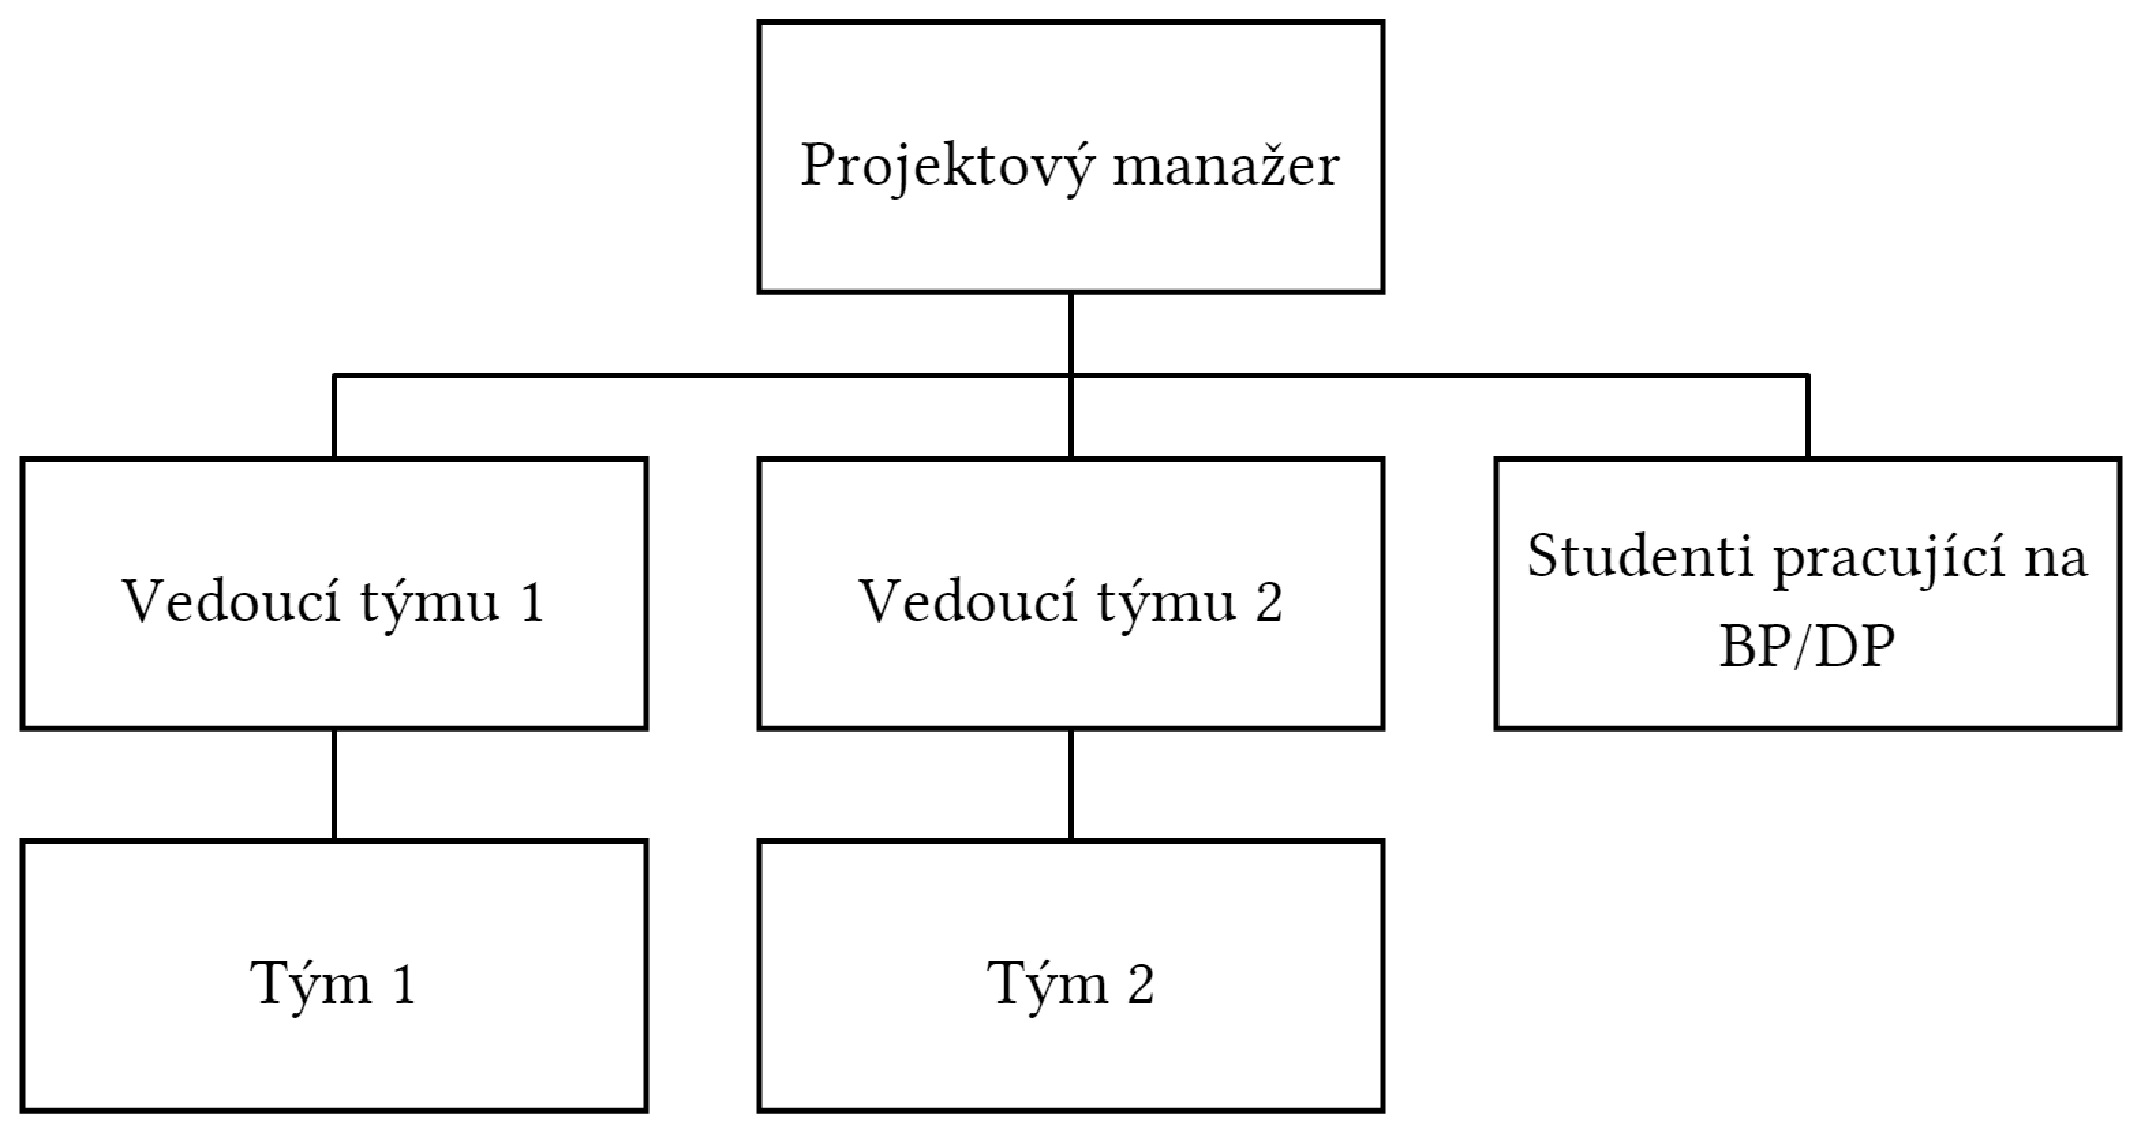
\includegraphics[width=\textwidth]{../pdf/dbs-obs.pdf}
\caption{Organization Breakdown Structure používaná v DBS projektu} \label{picture:obs}
\end{figure}
Je však nutné přiznat, že tato struktura v případě našeho projektu vznikla spíše \emph{na základě dostupných lidí}, než naopak. Dělení na týmy fungovalo již od začátku, vedoucí týmu však často nezvládal plnit práci, která po něm byla požadována. Teprve po dalším zastřešení jejich zodpovědnosti \emph{projektovým manažerem} se stala pozice vedoucího týmu důležitější, a to především na úrovni komunikace manažera s týmem. Veškeré úkoly, které manažer do týmu zadává, prochází přes vedoucího týmu, který práci dále rozděluje, a po jejím dokončení opět kontroluje. Tento proces je znázorněn i na activity diagramu v příloze \ref{picture:activity}.

%%%%%%%%%%%%%%%%%%%%%%%%%%%%%%
%%%%%%%%%%%%%%%%%%%%%%%%%%%%%%
%%%%%%%%%%%%%%%%%%%%%%%%%%%%%%

\section{Zajištění projektového týmu}

Tento proces se primárně stará o \emph{příjem nových pracovníků}, \emph{řízení jejich vytížení} a \emph{vyrovnání}. První ze zmíněných je především v IT hodně diskutované téma, kdy najít člověka se správnou kvalifikací je často nadlidský úkol. Firmy se tak přetahují, kdo nabídne zajímavější pracovní prostředí, lepší benefity či \emph{evergreen}: vyšší plat.\\
Když už je \emph{ten správný} zaměstnanec přijat, je potřeba řídit jeho \emph{vytížení} a případně jeho vznik \emph{vyrovnávat}. Jedná se o metodiky, při kterých je sledováno množství práce zadané zaměstnanci, a v případě, že je po něm požadováno více, než je schopen zvládnout, je buďto přehodnocen harmonogram a úkoly s nižší prioritou jsou odloženy na později, nebo je k úkolu přiřazen další pracovník.\\
Plánování přiřazení práce je důležité především z důvodu předcházení výkyvů v množství přidělené práce, což vede k většímu pohodlí zaměstnance a také snadnějšímu řízení.

\subsection{Použití v DBS projektu}
Jelikož u DBS projektu se pohybujeme na akademické půdě a nikoliv ve světě byznysu, je zde přístup k náboru nových pracovníků trochu odlišný. Noví pracovníci - studenti - jsou sháněni jednak nárazově jednou ročně - při startu nového letního semestru - jednak kontinuálně - jakožto zájemci o bakalářskou či diplomovou práci.\\
První ze zmíněného náboru vyžaduje vypsání tématu na stránku předmětu BI-SP1, kde se snažíme studenty nalákat právě k našemu projektu. Především v tomto roce (2017) se zvýšila zajímavost ostatních nabízených projektů (různé mobilní aplikace atp.), a tak se i zde začal projevovat podobný efekt jako u reálných firem: \emph{lov pracovníků}. Zároveň jsme však po nových studentech chtěli, aby měli buď zkušenost s použitými technologiemi, nebo měli předpoklad k rychlému naučení těchto - pro někoho nových - technologií. Z toho důvodu jsme připravili \emph{vstupní kvíz} (viz níže podsekce \nameref{DBSmanagement:quiz}), který měl původně sloužit jako nutný požadavek pro vstup do týmů, z důvodu nízkého zájmu však byla poté jeho role přehodnocena. Kvíz byl studentům zadán až po jejich vstupu do projektu a na základě jejich výsledků byli rozděleni do podobně schopných týmů a také byli určeni vedoucí týmů - ti, kteří vykazovali nejvyšší aktivitu a zároveň nejlépe zpracovali kvíz.

\paragraph{Vstupní kvíz} \label{DBSmanagement:quiz}
\begin{quote}
Jedná se o malou aplikaci v Nette, která obsahuje 3 jednoduché úkoly s možností pokročilého rozšíření řešení. Ukázky kvízu jsou dostupné v příloze \ref{ap:quiz}.\\
Studenti si museli na svém počítači nainstalovat a nastavit webserver a stáhnout zdrojové kódy ze školního Gitlabu. Databáze se vytvořila sama při prvním spuštění - pro potřeby kvízu stačil databázový stroj SQLite. Následně byl student přihlášen do \emph{kostry aplikace}, která obsahovala 3 úkoly:
\begin{itemize}
	\item Zobrazování dat z databáze v tabulce a práci se zobrazováním data a času v čitelné formě.
	\item Jednoduché CMS: Přidávání, úprava a mazání příspěvků.
	\item Práce s komponentou Grido: Přidání sloupce tabulky, nastavení řazení, přidání akce.
\end{itemize}
Všechny tyto úkoly měly navíc \emph{volitelé} rozšíření, které se většinou zaměřovalo na korektní návrh architektury MVP. 
\end{quote}

Druhým náborem, který probíhá neustále, je nábor studentů, kteří budou na projektu pracovat v rámci své bakalářské či diplomové práci. Takoví studenti zpravidla přichází sami s požadavkem o vymyšlení tématu BP/DP či zůstávají u projektu po skončení jejich působení v předmětu BI-SP2. Tito studenti vyžadují zpravidla méně \uv{péče} projektového manažera, protože již vědí, co chtějí realizovat, a často jsou v daném tématu i zběhlejší než já. Běžně také svou práci spíše než se mnou konzultují s Jiřím Hunkou - který vede nejen realizační týmy SP1/SP2, ale také právě bakalářské a diplomové práce.\\

Kromě nabírání nových lidí patří do tohoto procesu také řízení jejich vytížení a vyvažování přidělené práce. Jak vyplývá z obrázku \ref{picture:obs}, já jakožto projektový manažer se nestarám přímo o zátěže jednotlivých členů týmu, ale práci přiděluji pouze týmům jako celkům. Rozdělení práce v týmu je plně v kompentenci týmových vedoucích, což dále rozvíjí jejich schopnosti vést tým. Pro správu přidělené práce využíváme \emph{Redmine}, jehož použití se více věnuji v kapitole \ref{if:redmine}.

%%%%%%%%%%%%%%%%%%%%%%%%%%%%%%
%%%%%%%%%%%%%%%%%%%%%%%%%%%%%%
%%%%%%%%%%%%%%%%%%%%%%%%%%%%%%

\section{Rozvoj projektového týmu}

V předchozí sekci jsme zajistili vznik týmu, tím však zdaleka práce nekončí. Hned po vytvoření týmu se spouští jednotlivé fáze vývoje týmu, jak je definoval \emph{Tuckman} \cite{tuckman} v roce 1965:
\begin{enumerate}
	\item \emph{Forming (formování)}\\Při samotném vzniku nebo při příchodu nového člena dochází k představování, určování rolí v týmu atp. Většinou není během této fáze vyprodukována žádná práce, ale jedná se o nedílnou součást vývoje týmu, která nemůže být opomenuta.
	\item \emph{Storming (krize)}\\Jakmile jsou stanoveny role v týmu a začíná samotná práce, začne docházet k nedorozuměním, ujasňování rolí, odpovědností a kladených požadavků na jednotlivé členy. Toto zákonitě přináší jisté rozepře, které musí tým řešit.
	\item \emph{Norming (stabilizace)}\\Pokud jsou rozepře z předchozí fáze vývoje týmu úspěšně vyřešeny, dostává se tým do fáze stabilizace, ve které dochází k vyjasnění a vylepšení komunikace týmu a tím i jeho výkonnosti.
	\item \emph{Performing (optimální výkon)}\\Po průchodu všemi předchozími fázemi se tým dostává na vrchol své výkonnosti, je schopen zvládnout mnohem složitější úkoly a má stabilizované vnitřní vztahy.
\end{enumerate}
Kromě těchto čtyř základních fází je vhodné zmínit ještě dvě doplňující, a to \emph{rozpad týmu}, který může nastat po neúspěšném \emph{stormingu} a který buďto vede k ukončení celého projektu nebo přeskupení členů týmu - pokud to povaha projektu dovoluje. Poté nastává opět první fáze \emph{forming} s novým členěním týmu. Druhou doplňující fází je \emph{rozpuštění týmu}, která nastává po skončení projektu.

\subsection{Školení}
Další součástí rozvoje týmu je školení pracovníků v nových dovednostech. Firmy často nabízejí svým zaměstnancům možnost účastnit se různých kurzů, ať už s lektorem, nebo ve formě e-learningu. Tyto kurzy by měly být vhodně plánovány s ohledem na nadcházející práci, která bude zaměstnancům zadávána. V opačném případě se budou školení míjet účinkem a ponesou tak pouze náklady.

\subsection{Systém odměňování a oceňování}
Důležitou součástí je také odměňování lidí. Typicky jsou speciálně odměňováni ti pracovníci, kteří řeší úkoly nad rámec zadání nebo ve svém volném čase pomáhají kolegům s jejich prací. Odměny mohou být finanční nebo mít například podobu delší dovolené. Pro manažera je důležité správně rozlišovat práci vykonanou navíc a kladně ji hodnotit, tak aby byli pracovníci dostatečně motivováni. Nesmí však docházet k jevu, kdy pracovníci dělají práci navíc \emph{pouze} pro získání zmíněných bonusů.

\subsection{Použití v DBS projektu}
Proces rozvoje projektového týmu má několik částí, i jejich použití v DBS projektu si tedy pro lepší přehlednost rozčleníme.

\subsubsection{Rozvoj projektového týmu}
Čtyři fáze vývoje týmu popisované výše probíhají i v týmech, které programují DBS portál. Zvláště v letním semestru 2017, kdy vznikala tato práce, byly rozdíly mezi týmy velmi dobře sledovatelné, a to díky jejich rozdílenému složení:
\begin{itemize}
	\item \emph{Team 1} vznikl spojením 5 studentů, kteří se do té doby vůbec neznali. U tohoto týmu byla patrná především první fáze \emph{formingu}, kde byli jednotliví členové rozpačití, nevěděli, co si mohou dovolit, a vedoucí byl ve své pozici nejistý. V průběhu následujících týdnů se však stav výrazně zlepšil a tým je nyní schopen provádět i komplexnější úlohy a rozvrhnout si práci. Předpokladem je, že do následujícího semestru, kdy budou studenti na projektu pracovat v rámci BI-SP2, dosáhne tým fáze \emph{performingu} a jeho výstup bude na vysoké úrovni.
	\item \emph{Team 2} na rozdíl od prvního týmu vznikl ze 4 studentů, kteří se již před začátkem projektu znali. Měli jasně zvoleného vedoucího, který byl zároveň nejzkušenějším z nich. U tohoto týmu tak vůbec neproběhly fáze \emph{forming}, \emph{storming} ani \emph{norming} a nebylo tak možné se dostat k nejefektivnější poslední fázi: \emph{performing}. V době psaní této práce bylo nejvíce práce ve druhém týmu vykazováno právě vedoucím, který sice opravdu zkušený byl a jeho výstup byl kvalitní, nezvládl ale dovést svůj tým k optimálnímu výkonu. To znamenalo, že ostatní členové často záviseli právě na svém vedoucím, který \uv{zařídil vše}. Já, jakožto manažer projektu, se snažím do tohoto rozložení zasáhnout, aby se i team 2 dostal do své nejefektivnější fáze, a doufám, že do příštího semestru se mi podaří tohoto cíle dosáhnout.
\end{itemize}
Když tedy porovnáme tyto dva týmy, dostáváme se k jednoduchému závěru: \emph{Team 1}, přestože ze začátku byl v rozpacích a jeho výstupy byly slabší než týmu druhého se postupem času díky průchodu jednotlivými fázemi dostal do lepší pozice. Naopak \emph{Team 2} začal díky svému zkušenému vedoucímu vykazovat hned od začátku kvalitní práci, dá se však předpokládat, že pokud nedojde k zásadní změně v rozložení týmu, nebude se již tato efektivita zvyšovat, naopak se dá očekávat i její pokles.

V době dokončování této práce se navíc vedoucí Teamu 2 dozvěděl, že kvůli neúspěšné zkoušce odložené do LS nemůže dále pokračovat ve studiu. Podle posledních informací by měl však pokračovat s vedením svého týmu minimálně do konce tohoto semestru, na semestr příští si však budou muset zbývající členové zvolit mezi sebou nového vedoucího.

\subsubsection{Školení}
Na začátku letního semestru, kdy se k projektu dostávají noví studenti, jsou kromě úvodu do projektu pořádána i dodatečná školení, především týkající se použité technologe - Nette Frameworku, ale také například zaměřená na Git či různá \uv{how-to}, která jsou užitečná při vývoji DBS portálu.\\
Tato školení jsou většinou pořádána studenty, kteří na projektu pracovali v minulosti v rámci předmětů BI-SP1/2 a u projektu zůstali v rámci svých BP či DP.\\
Jelikož letošní rok bylo školení pořádáno hned ve druhém týdnu semestru, studenti byli ještě rozpačití a ostýchali se pokládat dotazy ohledně věcí, které by je zajímaly. Z toho důvodu jsem se školení také zúčastnil, přestože v roli lektorů již byli Pavel Kovář a Milan Vlasák, kteří také pracovali na BP týkajících se DBS portálu. Já jsem tedy měl příležitost zúčastnit se jako posluchač, čímž jsem se snažil přiblížit \uv{druhé straně bariéry} - novým studentům - a schválně jsem kladl i \emph{základní dotazy}, které jsem považoval za vhodné právě pro nové týmy. Mým cílem tedy bylo jednak navodit přátelskou atmosféru - ve které je možné zeptat se na cokoliv - jednak \uv{rozbít} \emph{groupthink} a \emph{konformitu s většinou}, jak je definoval Procházka \cite{prochazka} ve své lekci \emph{Skupinová dynamika, Týmová spolupráce} v kurzu \emph{Manažerské psychologie}, které jsem se zúčastnil v zimním semestru 2015.
\paragraph{Groupthink, konformita s většinou}
První zmíněný, v překladu \emph{skupinové myšlení}, je jev, který nastává při neřízené debatě několika, i velmi inteligentních, lidí. Při groupthinku může taková skupina dojít i ke zcela špatným rozhodnutím, neboť nikdo nechce vystupovat jako \uv{černá ovce} a rozbít skupinový souhlas, všichni tak \emph{v tichosti} odsouhlasí první návrh, který padl. Často se stává problémem, že osoba ve vůdčí pozici vyjádří svůj názor a poté se zeptá na názor podřízených. Ti ve valné většině budou pouze souhlasit, jelikož je jim nepříjemné vystoupit proti názoru jejich nadřízeného. Kdyby však byl nejprve dán prostor pro vyjádření podřízených a poté prezentována představa vedení, existuje mnohem větší šance, že budou probrány všechny aspekty řešeného problému. Pro prevenci groupthinku je vhodné do každé debaty zařadit alespoň jednoho \emph{rozvraceče}, jehož úkolem bude zpochybňovat veškeré názory a rozvířit tak mnohem produktivnější diskuzi.\\
Konformita s většinou je podobný jev jako groupthink a nastává ve chvíli, kdy v určité skupině lidí většina zastává nějaký názor. Člověk, který si myslí něco jiného, se pak velmi často \emph{přizpůsobí} většině, z důvodu \uv{aby nebyl divný}, aby si ostatní \uv{něco nemysleli} atp. Průzkumy \cite{prochazka} ukázaly, že stačí 3-4 další osoby, které mohou tvrdit i naprostý nesmysl, a nezávislá další osoba se i přes vnitřní nevoli velmi často \emph{přizpůsobí většině}. Při kladení sady otázek, kde 4 figuranti schválně odpovídali špatně, se 32\% osob přizpůsobilo jejich \emph{špatné} odpovědi pokaždé, 74\% se přizpůsobilo alespoň u jedné otázky. Stačí však jedna další osoba, která bude odpovídat \emph{jinak než většina}, a konformita rázem klesá na pouhých 6\% - přesně to bylo i mým cílem u školení nových studentů: aby se nebáli klást otázky, přestože většina studentů jen \emph{kývala}.

\subsubsection{Systém odměňování a oceňování} \label{ppl:ranking}
Odměnou, kterou student získává za práci na projektu, je především známka do předmětu BI-SP1/(BI-SP2) a také zápočet do předmětu BI-SI1. Tato známka se odvíjí od výsledků, kterých student při vývoji projektu dosahoval.\\
Hodnocení probíhá na dvou úrovních:
\begin{enumerate}
	\item Hodnocení týmu jako celku, udělované projektovým manažerem.
	\item Hodnocení jednotlivce v rámci týmu, udělované vedoucím týmu.
\end{enumerate}
První ze zmíněného uděluje manažer projektu a skládá se z následujících položek:
\begin{itemize}
	\item \emph{Vypracování přiděleného úkolu}\\Každý úkol, který je do týmů přiřazen, má nastavené body, které za něj lze získat. Výši bodů určuje manažer projektu (= zadavatel úkolu) a v případě odhalení vyšší obtížnosti v průběhu řešení úkolu mohou být body ještě dodatečně upraveny, nikdy však sníženy. Proces vypracování úkolu popisuje \nameref{picture:activity} dostupný v příloze \ref{picture:activity}. Výsledné hodnocení úkolů je definováno v tabulce \ref{table:ranking}.
	\begin{table}[h]
		\caption{Bodování týmů dle míry splnění úkolu}
		\label{table:ranking}
		\begin{tabular}{@{}ll@{}}
			\toprule
			Míra splnění úkolu                                                                           & Bodový zisk \\ \midrule
			Úkol splněn nad rámec zadání                                                                 & 125\% bodů  \\
			Úkol plně splněn, funguje                                                                    & 100\% bodů  \\
			Úkol splněn, má malé nedostatky (ale lze nasadit)                                            & 75\% bodů   \\
			Úkol splněn pouze z části, lze nasadit                                                       & 50\% bodů   \\
			Úkol řešen, je vidět náznak (správného) řešení,\\ale výsledek nefunguje (nelze nasadit)      & 25\% bodů   \\
			Úkol není na Gitu, není nastaven jako vyřešený\\v Redmine nebo řešení absolutně nelze použít & 0 bodů   \\ \bottomrule
		\end{tabular}
	\end{table}
	\item \emph{Nahlášení nového úkolu}\\Studenti jsou vedeni k vlastní iniciativě. Když přijdou s novým úkolem, který vede ke zlepšení výsledné aplikace nebo opravuje závažnou, dosud nenahlášenou chybu, je jejich tým kladně ohodnocen.
	\item \emph{Práce vedoucího týmu}\\Jelikož vedoucí týmu má za úkol nejen sám pracovat na úkolech, ale i rozdělovat práci, kontrolovat výstupy svého týmu a řídit komunikaci, je každý týden hodnocen i za tuto práci. Manažer tedy sleduje aktivitu vedoucího především na Slacku a Redmine a jednou týdně vyhodnotí kvalitu jeho práce. Získané body se také počítají jako zisk celého týmu.
\end{itemize}

Výše popsané možnosti získávání bodů přináší body vždy celému týmu a jednotlivým členům jsou rovnoměrně rozdistribuovány. Vedoucí týmů však mají ještě možnost hodnotit svůj tým interně, a to jak uznají za vhodné. Jedinou podmínkou je, že součet bodů udělených v týmu se musí vždy rovnat nule, pokud má tedy některý člen týmu získat plusové body, musí být body odebrány jinému členovi. Manažer projektu se snaží do tohoto interního hodnocení týmů nezasahovat, ale kontroluje například, zda není některý člen cíleně utlačován.\\

Tabulka hodnocení týmů v letním semestru 2017 je dostupná v příloze \ref{ap:ranking}.

%%%%%%%%%%%%%%%%%%%%%%%%%%%%%%
%%%%%%%%%%%%%%%%%%%%%%%%%%%%%%
%%%%%%%%%%%%%%%%%%%%%%%%%%%%%%

\section{Řízení projektového týmu}

Zbývá poslední proces řízení lidských zdrojů, a to \emph{řízení projektového týmu}. To velmi často probíhá pomocí tzv. \emph{soft skills} neboli měkkých dovedností, jelikož je zde potřeba sledovat rozhovory a mezilidské vztahy, hodnotit výkonnost projektu, řešit konflitky atp.\\
Mezi hlavní problémy, ke kterým může docházet, lze zařadit:
\begin{itemize}
	\item nedostatek důvěry,
	\item strach z konfliktů,
	\item nedostatek zapojení,
	\item vyhýbání se zodpovědnosti,
	\item lhostejnost k výsledkům.
\end{itemize}
Cílem manažera by mělo být snažit se tyto problémy řešit, či ještě lépe, zařídit, aby k nim vůbec nedocházelo.

\subsection{Použití v DBS projektu} \label{DBSmanagement:meeting}
Při řízení DBS projektu se snažím předcházet výše zmíněným problémům pomocí následujících technik:
\begin{itemize}
	\item Studenti jsou vedeni k vyjadřování vlastních názorů, snažíme se být otevřeni jakýmkoliv návrhům včetně kritiky vedení. Ze zkušeností vyplývá, že je toto pro studenty často jednodušší vyjádřit při osobní konzultaci, nikoliv při schůzce, kdy poslouchají i všichni ostatní členové. Po skončení úvodní \uv{společné} části schůzky tedy začínám obcházet jednotlivé studenty a ptám se na jejich problémy, názory atp.
	\item Hodnocení výsledků je transparentní, snažím se o jeho smysluplnost a srozumitelnost. Každý vidí, kolik za svůj úkol získal bodů, a také, kolik bodů získávají ostatní členové. To by mělo napomáhat snížit lhostejnost k \emph{bodovým} výsledkům, stále však přetrvává problém lhostejnosti k \emph{softwarovým} výsledkům. Stává se, že někdy je úkol vyřešen pouze \uv{tak, aby splňoval zadání} a výsledné funkčnosti poté schází jednoduchost při používání cílovým uživatelem. Tomuto problému se snažím předcházet zvýšením bodového hodnocení za velmi kvalitní řešení úkolu, hlavním problémem však je, že programátoři zároveň nejsou uživatelé systému. Pokud by tomu tak bylo, kvalita UI a UX by šla výrazně nahoru, protože by samotné autory aplikace \emph{rozčilovalo} její používání. Tento cíl však není efektivně realizovatelný, protože předmět, na který systém cílí, mají již tito studenti absolvovaný a pro roli učitele zase nemají dostatečnou kompetenci. Často tak chyby v použitelnosti nahlašují až koncoví uživatelé, a to především Jiří Hunka.
\end{itemize}



\paragraph{Softwarová podpora řízení lidských zdrojů}

Pro řízení projektu používáme mnohé podpůrné programy a aplikace. Této problematice se více věnuje samostatná kapitola \ref{infrastructure}.
